\documentclass[10pt,journal,compsoc]{IEEEtran}
\IEEEoverridecommandlockouts
% The preceding line is only needed to identify funding in the first footnote. If that is unneeded, please comment it out.
\usepackage{cite}
\usepackage{amsmath,amssymb,amsfonts}
\usepackage{algorithmic}
\usepackage{graphicx}
\usepackage{textcomp}
\usepackage{xcolor}

\def\BibTeX{{\rm B\kern-.05em{\sc i\kern-.025em b}\kern-.08em
    T\kern-.1667em\lower.7ex\hbox{E}\kern-.125emX}}
\begin{document}

\title{Conference Paper Title\\
    % {\footnotesize \textsuperscript{*}Note: Sub-titles are not captured in Xplore and
    % should not be used}
    % \thanks{Identify applicable funding agency here. If none, delete this.}
}
\author{}
% \author{\IEEEauthorblockN{1\textsuperscript{st} Given Name Surname}
% \IEEEauthorblockA{\textit{dept. name of organization (of Aff.)} \\
% \textit{name of organization (of Aff.)}\\
% City, Country \\
% email address or ORCID}
% \and
% \IEEEauthorblockN{2\textsuperscript{nd} Given Name Surname}
% \IEEEauthorblockA{\textit{dept. name of organization (of Aff.)} \\
% \textit{name of organization (of Aff.)}\\
% City, Country \\
% email address or ORCID}

\maketitle

\begin{abstract}
    This document is a model and instructions for \LaTeX.
    This and the IEEEtran.cls file define the components of your paper [title, text, heads, etc.]. *CRITICAL: Do Not Use Symbols, Special Characters, Footnotes,
    or Math in Paper Title or Abstract.
\end{abstract}

\section{Introduction}
A common practice to gauge patients' physiological condition and acute clinical stability is using basic homeostatic measures like vital signs, haematologic findings, and neurological examinations. Various early warning systems have been proposed that use these measurements to assess whether patients face an imminent risk of deterioration or death [Smith13].

The National Early Warning Score (NEWS), developed in conjunction with the Royal College of Physicians, has been widely implemented across the NHS and by healthcare providers outside the UK [RCP17, pp.13]. It is a points-based early warning system to identify clinical deterioration in acutely ill patients based on routinely recorded vital signs: pulse, breathing rate, blood pressure, blood oxygen level, level of consciousness, and temperature. The paper-based NEWS allocates points in a weighted manner based on these measurements. The sum of these points, which makes up the patient's aggregate NEW score, is associated with "triggers" - thresholds that correspond to recommended levels of clinical response and monitoring frequency.

While initially designed to monitor for deterioration in secondary-care, the NEWS has been widely tested and validated across healthcare settings. In its latest revision of the standard, the RCP recommended that the NEWS also be used in emergency departments to "aid the initial assessment of patiens, ongoing monitoring and patient triage decisions" [RCP17, pp.18].

Across studies, the NEWS has been found to perform well in discriminating ward patients at risk of death, critical care admission, or cardiac arrest. The present report introduces the novel SCI dataset, which contains records of adult patients with acute or medical presentation at the Salford Royal NHS Foundation Trust from 2014-2022. We then use this dataset to assess the performance of NEWS in predicting adverse patient outcomes, such as those mentioned above, in the dataset population.

\section{Methodology}
\subsection{Data Collection and Contents}
The SCI dataset is collated from EPR records collected in real time from admissions to acute beds between 1st April 2014 and 31st March 2022. Further, the dataset includes administrative data produced in retrospect for financial (tarrif) purposes.

Our dataset includes records of patients who received ambulatory emergency care (AEC) or same-day emergency care (SDEC) and were discharged before midnight on the day of admission [NHS18]. AEC, alongside the medical admissions unit (EAU)  are the two common entry points for adult patients with general medical emergencies. Exceptions present in our records include certain booked admissions and patients directly transferred and admitted to medical or critical care wards.

As a routine part of admission, the responsible staff member (nurse or support worker) records the patient's vital signs withing $\sim 30$ minutes of arrival. The vital signs that make up the NEWS are measured simultaneously, in a standardised manner, using Dinamap monitors. The readings are manually transcribed into EPR and onto the patient's paper chart. Specifically, this data includes:
\begin{itemize}
    \item Body temperature ($^{\circ}$C)
    \item Pulse (beats/min)
    \item Diastolic and systolic blood pressure (mmHg)
    \item Peripheral oxygen saturation (\%)
\end{itemize}
Further, we record the patient's level of consciousness (AVPU), presence of pain, nausea, or vomiting, whether the patient was receiving oxygen at the time of SpO2 measurement and, if applicable, the oxygen flow-rate and mode of delivery. Once these parameters are inputted into EPR, the NEWS score and component sub-scores are automatically computed for the patient. Blood test results (including VBG), where those were peformed, are automatically recorded in the laboratory information management system LIMS) and subsequently imported into EPR.

Other patient information recorded on admission includes: Patient identifier data such as their unique patient number, age, sex, and address. Admission method (e.g., emergency A\&E, emergency GP referral, etc), their presenting complaint, arrival time, and the main A\&E diagnosis (following initial assessment).

Information gathered in retrospect includes the date and time of discharge, total length of stay (LOS), the wards the patient was admitted to (in chronological order) and the LOS per ward. Diagnoses coded using the ICD-10-CM standard are complied by a clinical coding team based on the existing codes and clinical notes recorded in EPR. Procedures and services are also recorded in detail in EPR, and are similarly coded in retrospect using the OPCS-4 standard.

\subsection{Outcomes} The outcomes we track are death during hospitalisation, death within 30 days after discharge, unanticipated admission to critical care, or unanticipated readmission to the same hospital. To assess the NEWS, we check for the occurrence of death or critical care admission within 24 hours, 48 hours, or at any point after the patient's arrival. For readmissions, we consider thresholds of 48 hours, 7 days, or 30 days after discharge.

Where it occurrs, patient death during their hospitalisation is identified from EPR. Mortality after discharge (within 30 days) is primarily determined from the regional primary care databases (Salford Integrated Records \& Greater Manchester Care Record). Critical care admission is identified from patients being admitted into the hospital's critical care unit (CCU) or the high-dependency medical unit (HH1M).

\subsection{Data Preparation} We perform all data manipulation in Python using the Numpy and Pandas libraries. As they are the only parameters that are transcribed manually into EPR, we check the patients' vital signs for spurious values against hard ranges (e.g., $0-100\%$ for SpO2) as well as soft thresholds that we base on the range of physiologically possible values as determined by professional clinical opinion. For parameters that have a recorded NEWS sub-score but their raw value is missing or marked as spurious, we infer the correct value as the midpoint of the relevant NEWS range. Where a parameter has a valid value but the NEWS sub-score is missing, we compute it in accordance with the specificaton [RCP17, pp.]. We use the same specification to compute the final NEWS score for any patients where this is not recorded in the original data. Full details of how each parameter is pre-processed are available in appendix A.

\subsection{Data Analysis} We assess the ability of NEWS to discriminate between patients who did and did not suffer an adverse outcome using AUROC (area under the ROC curve). We compute this using the scikit-Learn library. The minimum possible AUROC value is $0.5$ and corresponds to a completely random relationship between the score in question and the tracked outcomes. Generally, a score of $0.7-0.8$ indicates reasonable discrimination and values over $0.8$ indicate good discrimination.

We investigate the discriminative performance of both the raw NEWS score and the pre-defined "trigger" thresholds for low, medium, and high clinical risk (NEWS of $0-4$, $5-6$, and $\geq 7$ respectively) [RCP17, pp.30].

We measure correlation between ordinal variables (NEWS and LOS) using Spearman's rank correlation. We compare the means of independent samples of normally distributed variables using Welch's unequal variances t-test, and we use the Mann-Whitney U test for non-normally distributed variables. We present characteristics of variables as $mean \pm std$.

\section{Results}
\subsection{Population Characteristics} Records of $170833$ admissions were collated, of which $124162$ records, corresponding to $63450$ unique patients, had a NEW score recorded on-admission or computed by us during pre-processing. NEW scores ranges from $0-18$ with a median score of $1.0$ (IQR=$2.0$). Key characteristics of the dataset population are given in Table \ref{tab:population}.

\begin{table}[!t]
    \renewcommand{\arraystretch}{1.3}
    \centering
    \caption{SCI dataset key characteristics}
    \label{tab:population}
    \begin{tabular}{l l l}
        \hline\hline
        Parameter            & Category              & $n\;(\%)$           \\
        \hline
        Sex                  & Female                & $65096\;(52.43\%)$  \\\\
        Admission Method     & Emergency A\&E        & $113518\;(91.43\%)$ \\
                             & Emergency GP Referral & $5955\;(4.8\%)$     \\\\
        Admission Ward       & EAU                   & $82541\;(66.48\%)$  \\
                             & AEC                   & $36546\;(15.27\%)$  \\
                             & Other Medical         & $2980\;(2.4\%)$     \\
                             & High-Dependency       & $2095\;(1.69\%)$    \\\\
        Mortality            & No                    & $14768\;(92.43\%)$  \\
                             & Died During Stay      & $5308\;(4.28\%)$    \\
                             & Died within 30 Days   & $4086\;(3.29\%)$    \\\\
        Critical Care        & Yes                   & $4371\;(3.52\%)$    \\\\
        Readmitted (30 days) & Yes                   & $15836\;(12.75)$    \\\\
        NEWS clinical risk   & Low (0-4)             & $118223\;(95.1\%)$  \\
                             & Medium (5-6)          & $3748\;(3.02\%)$    \\
                             & High (>= 7)           & $2333\;(1.88\%)$    \\
        \hline\hline
    \end{tabular}
\end{table}

\subsection{Critical Event Occurrence} The original study on the NEWS' discriminative ability considered death within 24 hours of a given set of observations. We define a "Critical Events" as the occurrence of either critical care admission or death during the hospital spell. Since the vital signs and NEWS in our dataset are measured on admission, we investigate the subsets of hospital spells with total LOS within certain thresholds, such as 24 or 48 hours.

A total of $8826$ with recorded NEWS experienced a critical event, comprising $4371$ critical care admissions and $5308$ deaths. This was significantly correlated with the NEWS for the patient being over the defined threshold for high clinical risk ($p<0.0001$). The AUROCs ($95\%$ CI) of NEWS for critical events in records with 24h LOS, 48h LOS, or any LOS were respectively 0.914 (0.896-0.932), 0.890 (0.877-0.903), and 0.769 (0.763-0.775). The ROC curves are given in figure \ref{fig:criticalevent_roc}. The method for computing the AUROC confidence intervals is given in Appendix \ref{appendix:auroc}.

\begin{figure*}[htbp]
    \centering
    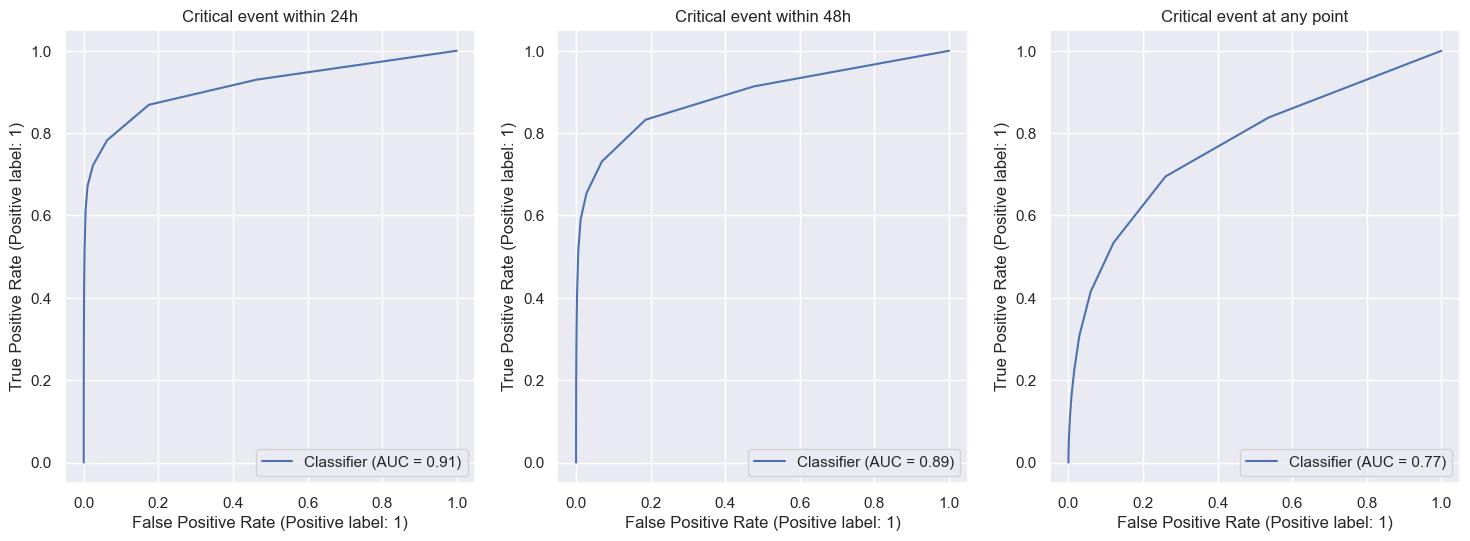
\includegraphics[width=\textwidth]{img/critical_event_roc.png}
    \caption{ROC curves of NEWS for discriminating critical event occurrence in stays with LOS under 24h (left), under 48h (middle), or any LOS (right).}
    \label{fig:criticalevent_roc}
\end{figure*}

Critical event occurrence significantly correlated with the NEWS at the same LOS thresholds: chi-square with NEWS $\geq 7$: $p < 0.0001$ in all cases. In total, $1423/8826 \; (16\%)$ of critical event occurrences had NEWS $\geq 7$. The full chi-square results are given in Appendix \ref{appendix:stats}. The same appendix gives the results for mortality and critical care admission examined separately.

Patients who experienced critical events were older ($71.72 \pm 16.85$ years; Welch's unequal variances t-test: $p < 0.0001$) and had higher NEWS ($3.51 \pm 3.1$; Mann-Whitney U test: $p < 0.0001$) compared to patients who did not (mean age $64.5 \pm 20.62$ years; NEWS $1.04 \pm 1.4$). The mean total LOS was $16.32 \pm 24.25$ for patients who experienced critical events and $6.07 \pm 13.62$ for those who did not (Mann-Whitney U test: $p < 0.0001$). Table \ref{tab:criticalevent_stats} gives the same information across the tested LOS thresholds.

\begin{table}[!t]
    \renewcommand{\arraystretch}{1.3}
    \centering
    \caption{Distribution comparison dep. on critical event occurrence.}
    \label{tab:criticalevent_stats}
    \begin{tabular}{l l l l l l}
        \hline\hline
        Variable & LOS & Mean (Event)      & Mean ($\lnot$Event) & Test  & $p$   \\
        \hline
        Age      & 24h & $71.4 \pm 18.92$  & $57.62 \pm 20.92$   & Welch & $0.0$ \\
                 & 48h & $70.54 \pm 19.56$ & $58.71 \pm 21.09$   &       & $0.0$ \\
                 & Any & $71.72 \pm 16.85$ & $64.5 \pm 20.62$    &       & $0.0$ \\
        NEWS     & 24h & $6.82 \pm 4.38$   & $0.75 \pm 1.07$     & Mann  & $0.0$ \\
                 & 48h & $5.91 \pm 4.18$   & $0.78 \pm 1.1$      &       & $0.0$ \\
                 & Any & $3.51 \pm 3.1$    & $1.04 \pm 1.4$      &       & $0.0$ \\
        \hline\hline
    \end{tabular}
\end{table}

\onecolumn
\appendices

\section{Data Pre-processing}
\label{appendix:preprocessing}

\section{AUROC}
\label{appendix:auroc}
We assess the discriminative ability of the NEWS using an area under the receiver-operating characteristics (AUROC) curve. This measurement is commonly used to assess the accuracy of a criterion variable whose value will be used to make a binary decision. We construct the ROC curve by plotting the false-positive rate ($1$ minus the specificity) on the x-axis against the true-positive rate (sensitivity) on the y-axis for each decision threshold for prediction between $0-100\%$. In our methodology, we use scikit-Learn for automatic plotting and AUC computation.

For large samples, the distribution of the AUC is approximately normal. Hence, we use the standard normal distribution to claculate the confidence interval for the AUC as:

\begin{equation}
    AUC \pm z_{\alpha/2}SE(AUC)
\end{equation}

The formula for $SE(AUC)$ is [Henley82]:

\begin{equation}
    SE(AUC) = \sqrt{\frac{AUC(1-AUC) + (N_1-1)(Q_1-AUC^2) + (N_2-1)(Q_2-AUC^2)}{N_1N_2}}
\end{equation}
where,

\begin{equation}
    Q_1 = \frac{AUC}{2-AUC}, \;
    Q_2 = \frac{2AUC^2}{1+AUC}
\end{equation}

\end{document}
